\documentclass[conference]{IEEEtran}
\IEEEoverridecommandlockouts
% The preceding line is only needed to identify funding in the first footnote. If that is unneeded, please comment it out.
\usepackage{cite}
\usepackage{amsmath,amssymb,amsfonts}
\usepackage{algorithm}
\usepackage{algorithmic}
\usepackage{graphicx}
\usepackage{textcomp}
\usepackage{xcolor}

\usepackage{stfloats}%added by jing

\def\BibTeX{{\rm B\kern-.05em{\sc i\kern-.025em b}\kern-.08em
    T\kern-.1667em\lower.7ex\hbox{E}\kern-.125emX}}
\begin{document}

\title{Contrastive Self-Supervised Learning on Crohn's Disease Detection\\
% {\footnotesize \textsuperscript{*}Note: Sub-titles are not captured in Xplore and
% should not be used}

% \thanks{Identify applicable funding agency here. If none, delete this.}
}

% \author[a]{Jing XING}
% \author[a]{Harold Mouchère}
% %\author[a]{Author C \thanks{Corresponding author: email@mail.com}}


\author{
\IEEEauthorblockN{1\textsuperscript{st} Jing XING}
\textit{South China University of Technology}\\
GuangZhou, China \\
\IEEEauthorblockA{\textit{Nantes Université, École Centrale Nantes, CNRS}\\
LS2N, UMR 6004, F-44000 Nantes, France\\
xjjsdsb@gmail.com}
\and
\IEEEauthorblockN{2\textsuperscript{nd} Harold Mouchère}
\IEEEauthorblockA{\textit{Nantes Université, École Centrale Nantes, CNRS}\\
LS2N, UMR 6004, F-44000 Nantes, France\\
harold.mouchere@univ-nantes.fr}
}

\maketitle

\begin{abstract}

Crohn's disease is a type of inflammatory bowel illness that is typically identified via computer-aided diagnosis (CAD), which employs images from wireless capsule endoscopy (WCE). While deep learning has recently made significant advancements in Crohn's disease detection, its performance is still constrained by limited labeled data. We suggest using contrastive self-supervised learning methods to address these difficulties  which was barely used in detection of Crohn's disease. 
Besides, we discovered that, unlike supervised learning, it is difficult to monitor contrastive self-supervised pretraining process in real time. So we propose a method for evaluating the model during contrastive pretraining (EDCP) based on the Euclidean distance of the sample representation, so that the model can be monitored during pretraining.
Our comprehensive experiment results show that with contrastive self-supervised learning, better results in Crohn's disease detection can be obtained.
EDCP has also been shown to reflect the model's training progress. Furthermore, we discovered some intriguing issues with using contrastive self-supervised learning for small dataset tasks in our experiments that merit further investigation.
\end{abstract}

\begin{IEEEkeywords}
Deep Learning, Self-Supervised Learning, Contrastive Learning, Crohn's Disease, Medical images classification
\end{IEEEkeywords}

\section{INTRODUCTION}
Crohn's Disease is a common bowel disease\cite{capsule_Crohn}. 
Wireless Capsule Endoscopy (WCE) is commonly used by doctors to aid in diagnosis. However, counting and identifying lesions of Crohn's disease  in WCE videos is time-consuming. Many methods \cite{review_WCE_CNN} have been developed to automatically detect intestinal abnormalities in WCE images, such as ulcer, bleeding, and erosion.
These methods can be divided into two main categories. One is using Support Vector Machine(SVM)
%bejakovic2009analysis, karargyris2009identification, girgis2010intelligent,kumar2011assessment,
\cite{hajo2012segmentation,chen2012ulcer,charisis2012capsule,eid2013curvelet,szczypinski2014texture,yeh2014bleeding,iakovidis2014automatic,yuan2015saliency,charisis2016use,liaqat2018automated,alotaibi2013empirical,souaidi2019multi} with manually designed features. 
The other is based on deep learning\cite{georgakopoulos2016weakly,fan2018computer,aoki2019automatic,alaskar2019application,crohIPI,de2021multi}. 
In the early years, researchers primarily used SVM as classifiers based on manually designed features such as local binary pattern\cite{lbp_sift_bagOfWords_svm}, scale invariant feature transform\cite{lbp_sift_bagOfWords_svm}, texture feature\cite{saliencyMap_gabor_lbp_svm}, color feature\cite{colorFeature_3layerMLP}, etc. However, deep learning has demonstrated tremendous power in a number of fields in recent years. The accuracy of Crohn's disease detection has increased significantly with deep neural networks to over 90\% \cite{review_WCE_CNN}. 

As shown in Fig. \ref{fig:method}, the images for Crohn's disease detection are taken from WCE video, thus there are numerous unlabeled images. Nevertheless, because labeling WCE image is very time-consuming and requires professional doctors, labelled data is scarce.  As a result, deep learning's effectiveness in the field of medical images, including Crohn's disease detection, is massively diminished. In this situation, self-supervised learning is a viable option. Given that it can train the network with unlabeled data to make up for the lack of enough labeled data. Self-supervised methods based on contrastive learning have recently been proven to be more effective in image classification tasks.
\begin{figure*}[t]
\centerline{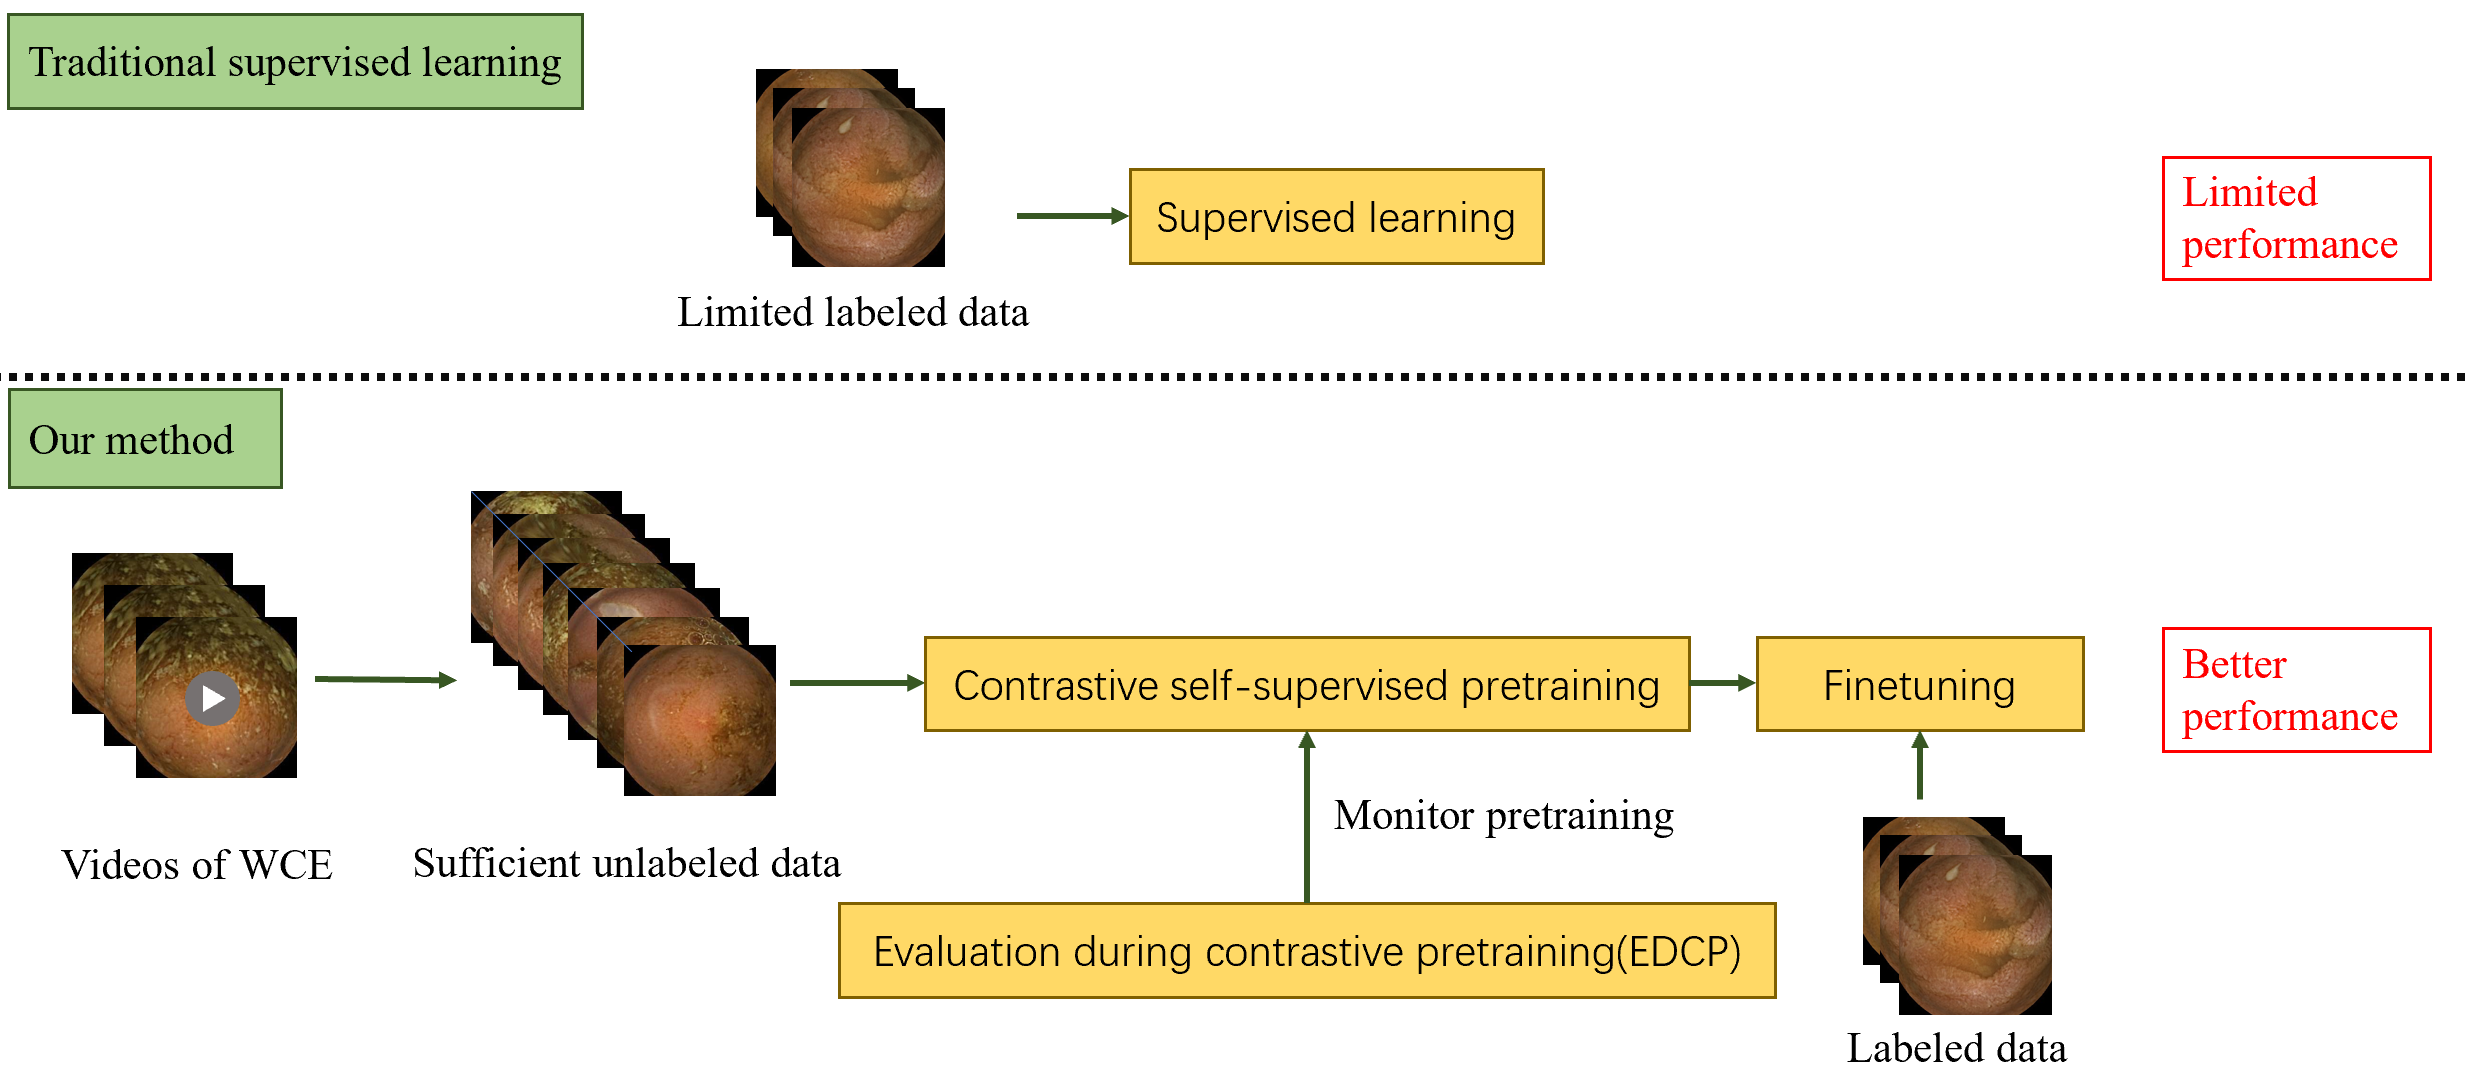
\includegraphics[scale=0.5]{images/method.png}}
\caption{Traditional supervised learning (top), our contrastive self-supervised learning method (bottom). Evaluation During Contrastive Pretraining(EDCP) is used to monitor pretraining(Bottom). The wireless capsule endoscopy (WCE) images are from CrohnIPI\cite{crohIPI}.}
\label{fig:method}
\end{figure*}
The CrohnIPI\cite{crohIPI} dataset that we use is a professional public dataset that contains well-labeled data.
To the best of our knowledge, existing research works use only self-supervised learning  for Crohn's disease detection. Besides, most self-supervised studies use very large datasets as benchmark, such as ImageNet \cite{deng2009imagenet}. However, WCE images are usually small and have few categories which is very different to ImageNet. Considering the gap between ImageNet and WCE images, we compare several state-of-the-art contrastive self-supervised learning methods' performance on WCE data to find out that whether self-supervised learning can improve the performance of Crohn's disease detection. 

During our experiments, we discovered that self-supervised training, also referred pretraining, unlike supervised training, cannot use the validation set to observe the pretraining process. This also makes selecting model of pretraining and conducting early-stopping impossible. We can only use finetuning to verify the model's performance after pretraining, which significantly prolongs the model's tuning process and makes selecting the best model during the pretraining process for downstream tasks difficult.
Therefore, we propose \textit{evaluation during contrastive pretraining} (EDCP), a low-cost method for real-time monitoring of pretraining progress. Based on the Euclidean distance between sample representations, this method computes a value that reflects how well network is trained. We compare the EDCP to the results of few-epoch finetuning and discovered that the EDCP results are consistent with the few-epoch finetuning results, which demonstrats that EDCP can be used effectively to monitor contrastive self-supervised learning pretraining.

Furthermore, we observed some contrastive learning techniques that are useful on large datasets but are ineffective or even harmful for Crohn's disease detection in experiments. A larger batch size, for example, will generally produce better results\cite{SimCLR}, but it has no effect on Crohn's disease detection, and even too many negative sample pairs will degrade the model's performance.
These anomalous phenomena merit further investigation, as they may improve the model's performance and have some reference significance for similar classification tasks of small dataset.

The following are our primary contributions: \textbf{(i)}We are the first to apply self-supervised learning to the detection of Crohn's disease in images. \textbf{(ii)} We outperform traditional supervised learning in the detection of Crohn's disease. \textbf{(iii)} We propose using evaluation during contrastive pretraining (EDCP) to track the progress of contrastive self-supervised training.
%\textbf{(iiii)} Some intriguing experimental results merit further investigation.

\section{PRELIMINARY AND RELATED WORK}
\label{sec:related work}
\textbf{Crohn's Disease Detection.}
 Computer-aided diagnosis (CAD) has become an active search area in the past few years. WCE is crucial for the diagnosis of Crohn's disease because it allows medical professionals to see inside the patient's bowel in order to identify Crohn's disease as soon as possible. However, diagnosing with WCE images takes a long time for medical experts.
Many methods for automatically detecting diseases in WCE based on deep learning have recently been proposed, and excellent results have been obtained \cite{review_WCE_CNN}.
Deep learning methods based on convolutional neural networks (CNN) have been proven to outperform prior machine learning methods which based on support vector machines (SVM) and manually designed features.
 However, there is still room for improvement due to the lack of labeled data. In fact, insufficient labeled data is a common issue in the medical imaging field. 
 For example, Segu{\'\i} et al\cite{segui2016generic} found that 10-fold cross-validation increase in training data size improved the accuracy by 3\% for motility movement classification in WCE.
WCE images have the significant advantage of being easy to obtain a large number of unlabeled images since tens of thousands of frames are contained in each WCE video. To make use of these unlabeled data, we employ self-supervised learning.


\textbf{Contrastive Self-Supervised Learning.}
Self-supervised learning (SSL) has recently achieved great success in a variety of fields.
Liu et al.\cite{review_generativeOrConstrasive} summarize the mainstream self-supervised learning into three broad categories: generative, contrastive, and generative-contrastive. 
In generative tasks such as image colorization \cite{colorization} and inpainting \cite{inpainting}, generative and generative-contrastive learning are particularly effective.
Contrastive learning, on the other hand, outperforms in classification tasks, particularly in computer versions (CV). Among contrastive learning methods, instance-instance contrast is proved perform better than context-instance contrast\cite{review_generativeOrConstrasive}. Many instance-instance\cite{he2019moco,SimCLR,moco_v2_chen2020improved,simclr_v2_chen2020big,BarlowTwins,BYOL,SwAV} have performed admirably on various CV benchmarks.
The object of contrast in contrastive learning is commonly referred to as negative samples and positive samples.
The different embeddings produced by transforming one image are referred to as positive samples from each other, whereas the embeddings produced by transforming different images are referred to as negative samples from each other. 
To obtain positive and negative samples, the contrastive learning network typically has two similar branches, and is therefore also known as siamese network\cite{simsiam}. 
The objective of contrastive learning is to maximize the similarity of negative pairs while minimize the similarity of positive pairs. 
InfoNCE\cite{CPC_Oord2018RepresentationLW} loss is commonly used to achieve this goal.
The InfoNCE loss for sample $q$ with distance measured by dot product is:

\begin{equation}
\label{equ:InfoNCE}
\mathcal{L}_{q}=-\log \frac{\exp \left(q \cdot k_{+} / \tau\right)}{\sum_{i=0}^{K} \exp \left(q \cdot k_{i} / \tau\right)},
\end{equation}
where $\tau$ is a temperature hyper-parameter. The sum is over one positive sample $k_+$ and $K$ negative samples. Many studies \cite{SimCLR,he2019moco,BarlowTwins} have shown that having a sufficient number of negative samples is critical for model performance and avoiding clloaps during pretraining.

\textbf{State of the Art (SOTA) Methods.}
 In the field of contrastive self-supervised learning, method iteration has been remarkably rapid in recent years. InvaSpread\cite{InvaSpread_Ye2019UnsupervisedEL} presents an end-to-end method for contrastive learning. 
Following InvaSpread, SimCLR made significant progress through refining the experiment and network structure including adding MLP head, more epochs of pretraining, much bigger batch size and more complex data augmentations. 
These manipulations are straightforward and effective, and they are followed by methods proposed later. 
Meanwhile, MoCo \cite{he2019moco} introduced momentum encoder to reduce inconsistency caused by rapidly changing encoder, based on InstDisc \cite{InstDisc_Wu2018UnsupervisedFL}, which proposed memory bank that use a small amount of computational resources while producing a large number of negative samples. 
MoCo v2 later combined the useful SimCLR strategies on the basis of moco to achieve better results.
Positive and negative pairs are sample-based in MoCo v2 and SimCLR, whereas in Barlow Twins \cite{BarlowTwins}, they are based on filters that generate embeddings. They believe that this will allow filters to learn more different features and reduce the redundancy of information.
Barlow Twins does not require a large batch size or memory bank, but it does require more channels in the MLP layer in order to obtain enough negative samples.
Most contrastive self-supervised learning methods proposed prior to BYOL \cite{BYOL} require negative samples to avoid trivial solutions. For example, if the network only needs to reduce the similarity of positive pairs, regardless of the input, the network can output the same feature vector. BYOL produces excellent results with only positive sample pairs and its performance is robust to small batch sizes.
Soon after, SimSiam\cite{simsiam} proposed a simplified version of BYOL which remove momentum encoder and the predictor head while slightly reducing performance.






\section{Methods}
\subsection{Baseline}
Our aim is to find out whether contrastive self-supervised learning can improve the performance of Crohn's disease detection. 
For comparison, the traditional supervised learning method is used. Following \cite{crohIPI}, the network structure of baseline consists of an encoder and a fully connected layer. The encoder is ResNet\cite{ResNet} without final fully connected layer. 
\subsection{Contrastive Self-Supervised Methods Comparison}

\begin{table}[tb]
\caption{Top-1 and top-5 accuracies (in \%) under linear evaluation on ImageNet. All models use ResNet-50 as encoder. The batch size is for pretraining. These results are come from corresponding papers.}
\centering
\begin{tabular}{llll}
\hline
Method      & Top-1 & Top-5 & Batch Size \\ \hline
Supervised  & 76.5  & -     & -          \\ \hline
MoCo        & 60.6  & -     & 256        \\
SimCLR      & 69.3  & 89.0  & 4096       \\
MoCo v2     & 71.1  & -     & 256        \\
SimSiam     & 71.3  & -     & 256        \\
Barlow Twins & 73.2  & 91.0  & 4096       \\
BYOL        & 74.3  & 91.6  & 4096       \\
 \hline
\end{tabular}
\label{tab;methods_comparison_linear_evaluation}
\end{table}
SOTA methods mentioned in \ref{sec:related work} can be divided into three categories according to the factors contrasted: positive and negative pairs based on instances(MoCo, MoCo v2, SimCLR, etc.), positive and negative pairs based on filters(Barlow Twins), and only positive pairs based on instances(BYOL, SimSiam). The best methods from each of these three categories for detecting Crohn's disease detection will be chosen.

We are primarily concerned with two aspects when comparing methods: performance and robustness to batch size.
A general comparison of the performance of self-supervised learning is to compare the performance of linear evaluation on ImageNet which is shown in Table \ref{tab;methods_comparison_linear_evaluation}. According to the Table \ref{tab;methods_comparison_linear_evaluation}, it can be seen that MoCo v2, SimSiam, Barlow Twins, and BYOL perform well. Barlow Twins and BYOL stand out among them.
When comparing the robustness of methods to batch size, the study\cite{BarlowTwins} in Barlow Twins shows that the performance of Barlow Twins and BYOL are still good when the batch size decreases, while the performance of SimCLR drop a lot. Because the loss strategy in the BYOL and Barlow twins determines that their performance is less dependent on a large number of negative samples.
MoCo v2's performance is also robust to batch size since its negative samples are primarily drawn from memory bank which is not influenced by batch size. 
As a result, three methods were chosen from the three categories based on their good performance and robustness of batch size: MoCo v2, BYOL, and Barlow Twins. Since the hyperparameters of each method are carefully tuned, we will try to keep the original hyperparameters of these methods during the experiment for fairness.

\subsection{Framework}
The three methods have similar structure which shown in the Fig. \ref{fig:architecture}.
\begin{figure*}[t]
\centerline{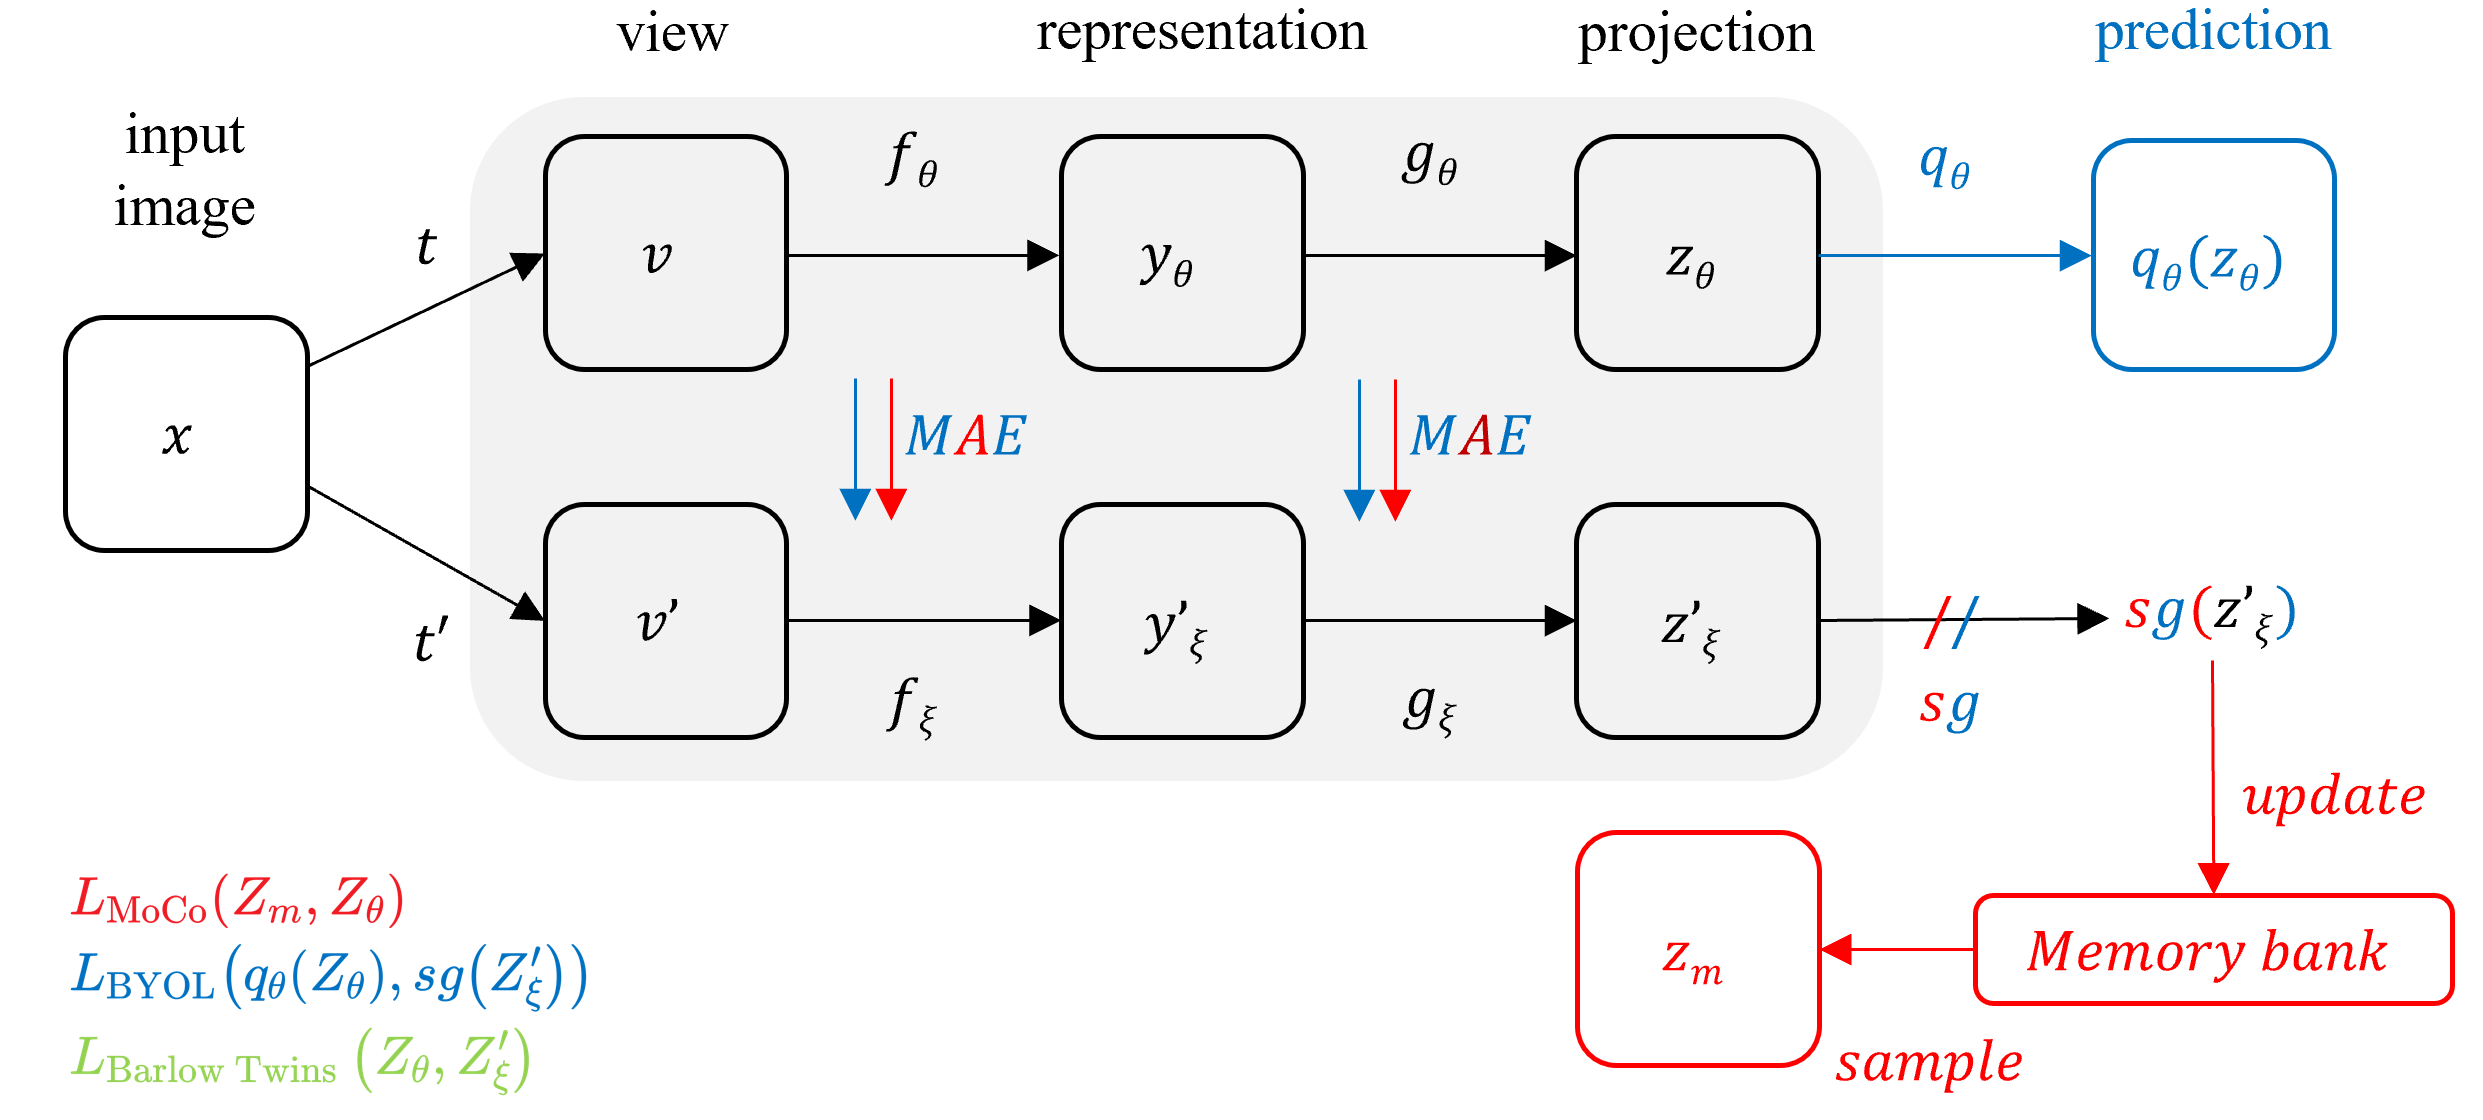
\includegraphics[scale=0.51]{images/frameworks.png}}
\caption{The architecture of MoCo v2, BYOL and Barlow Twins. The black part represents the structure shared by all three methods, the red part represents MoCo v2, and the blue part represents BYOL. $\theta$ are the trained weights, $\xi$ are exponential moving average of $\theta$ and $sg$ denotes stop-gradient. At the end of training, everything except  $f_\theta$ is discarded, and $y_\theta$ is used as the image representation. The embeddings used for calculating loss by three methods are shown in the lower left corner. }
\label{fig:architecture}
\end{figure*}
The input image is augmented $t$ and $t'$ to produce two distinct views for two branches. The network's goal is that the representations generated by two branches for two views of the same image are similar, while the representations generated for different input images are dissimilar.
The network, with the exception of the BYOL predictor, is made up of two symmetrical branches. Each branch is made up of an encoder $f$, which is a CNN followed by an projector network MLP.
The encoder structure of the three networks is ResNet without final full-connected layer, but the projector structure is different. The projector MLP structures of MoCo v2, BYOL, and Barlow Twins are 512-128, 4096-256, and 8192-8192-8192, respectively.
Following SimCLR, the projector MoCo v2 consists in a linear layer with output size 512 follwed by rectified linear units (ReLU) and a final linear layer with output dimension 256.
The projector of BYOL consists in a linear layer with output size 4096 followed by batch normalization, ReLU, and a final linear layer with output dimension 256. The predictor of BYOL uses the same architecture as projector.
The projector of Barlow Twins has three linear layers, each with 8192 output units. A batch normalization layer and ReLU are placed after the projector's first two layers.
We can see that Barlow Twins require large output dimension to provide a large number of negative samples in order to perform well. Besides, despite the simplicity of MoCo v2's MLP structure, MoCo v2 requires memory banks to provide a large number of embeddings as negative samples. 

The parameters of Barlow Twins are all updated by back-propagation.
However, in the network structure of BYOL and MoCo v2, the stop gradient operation is performed at the end of one branch, and the parameter $\xi$ of this branch is updated by exponential moving average (EMA) strategy which formulated by \eqref{equ:EMA}.Back-propagation updates the parameter $\theta$ of another branch.
 \begin{equation}\label{equ:EMA}
\xi \leftarrow \tau \xi+(1-\tau) \theta
\end{equation}
where $\tau\subset[0, 1)$ is a coefficient.

The embeddings used by the three methods to calculate the loss are different, as shown in the Fig. \ref{fig:architecture}.
MoCo v2 employs InfoNCE loss between projection $z_\theta$ and embedding $z_m$ sampled from the memory bank.
The loss in BYOL is calculated as the mean squared error between the $l2$-normalized projection $sg(z'_\xi)$ and the prediction $q_\theta(z_\theta)$.
After normalize the embeddings along the batch dimension,
Barlow Twins cleverly transposes one projection $z_\theta$ and multiplies it with another projection $z'_\xi$ to produce a cross-correlation matrix with diagonal and off-diagonal elements representing the cosine similarity of positive and negative sample pairs, respectively. The identity matrix is used as the label, and the loss is calculated as the mean square error of the cross-correlation matrix and the identity matrix in Barlow Twins.


\subsection{Evaluation During Contrastive Petraining (EDCP) }
The validation set is commonly used in supervised training to monitor training progress in order to avoid overfitting or insufficient training, and it can also be used to select models.
However, because the evaluation of self-supervised learning is finetuning when pretraining is finished, evaluating the network during pretraining is difficult.
Finetuning after each epoch during pretraining is a simple and straightforward method, but it adds a significant amount of time and computational resource consumption.
Another straightforward approach is to monitor pretraining process directly through observing the loss, but these losses are not related to the classification task.
First, this is an indirect method. There is inconsistency because the downstream task uses only the encoder rather than the entire pretraining network.
Second, the loss may gradually decrease with training due to the strategy of some methods. During pretraining, for example, the momentum of BYOL will gradually increase, resulting in closer parameters of the two branches of the network, which brings the generated representation closer to each other and eventually leads to a smaller loss.

To address this problem, we design a method for real-time monitoring of model training progress that can be quickly computed and widely used in any contrastive learning pretraining process, called evaluation during contrastive pretraining (EDCP). 

Based on the goal of contrastive learning, which is to decrease the positive sample pair's feature similarity close and increase the negative sample pair's feature similarity. Euclidean distance is used to measure similarity. We input a small amount of labeled data into the encoder to get the corresponding representations, and then calculate the Euclidean distance of the positive and negative sample pairs.
Two subsets are sampled with no overlap, each subset has the same number of samples with different labels, and they are converted into representations set $M, N$ by the encoder. Then subtract the distance of the negative representation pairs from the distance of the positive sample pair to get $S_{EDCP}$.
 For example, for a representation $m_{l}$ from $M$ with label $l$, find the closest representation $m_{l'}$ in $M$ with different label $l'$ and the closest representation $n_l$, $n_l'$ from $N$. Then use \eqref{equ:eval_distance3} to calculate the $L2$ distance of $m_{l}$ and other representations to get $d(m_{l},m_l')$,$d(m_{l},n_l)$ and $d(m_{l},n_l')$. Then subtract $d(m_{l},n_l')$ and $d(m_{l},m_l')$ by $d(m_{l},n_l)$ to get the distance value for $m_{l}$. Sum and all distance for each representation in ${M,N}$ will get $S_{EDCP}$. The calculation process is as follows:
\begin{equation}
\begin{aligned}
\label{equ:eval_distance1}
S_{EDCP}(M,N)=\frac{1}{K}[D(M,N)+D(N,M)]
\end{aligned}
\end{equation}

\begin{equation}
\label{equ:eval_distance2}
\begin{aligned}
D(M,N)=\sum_{i}[\min_{j}d( m_{i,l},n_{j,l} )  -\frac{1}{2}(\min_{j}d( m_{i,l},n_{j,l'} )\\+\min_{j}d(m_{i,l},m_{j,l'}))] 
\end{aligned}
\end{equation}
\begin{equation}
\label{equ:eval_distance3}
\begin{aligned}
d(m,n)=\left \| m-n \right \|_2
\end{aligned}
\end{equation}
Where $m_{l, i}$ is $i$-th sample of $M$ with label $l$, $n_{j,l}$ is $j$-th sample of $N$ with label $l$, $K$ is the sum number of ${M, N}$.

The smaller the value of $S_{EDCP}$, the better the encoder is trained. So that monitoring process of pretraining can be achieved by observing the curve of $S_{EDCP}$. And the encoder at the point where $S_{EDCP}$ reaches a minimum is likely to be the best pretrained encoder. 
Meanwhile, to assess if the trend of curve of $S_{EDCP}$ is correct, we conduct one-epoch-finetuning during pretraining. Because Crohn's disease detection is a relatively simple task that requires only a small number of epochs to complete finetuning, one-epoch-finetuning can, to some extent, represent the final result of finetuning at a lower cost. Therefore, the ability of EDCP to reflect the encoder's pretraining trend can be determined by comparing the results of EDCP and one-epoch-finetuning.


\section{Experiment}
To explore whether contrastive self-supervised learning can achieve better performance than traditional supervised learning on Crohn's disease detection, we first performed a baseline experiment to obtain results for comparison. Then, for each of the three contrastive self-supervised learning methods, perform pretraining and finetuning. The finetuning and baseline settings are the same. EDCP and one-epoch-finetuning are used during pretraining. All of our experiments were conducted on a 16GB Tesla T4.
\subsection{Dataset.} 
For baseline and finetuning experiments, 3484 labeled images of CrohnIPI\cite{crohIPI} are used, including 1360 pathological images and 2124 non-pathological images. For pretraining, 35053 unlabeled images were obtained from two WCE videos, different from the labeled images. It is worth noting that the majority of the datasets used in the WCE image detection task research are private datasets or unspecified subsets of public databases. However, CrohnIPI is a publicly available and well-labeled dataset that can be widely used as a benchmark for Crohn's disease detection.

\rm\subsection{Baseline \& Finetuning}



\textbf{Image Augmentations.}  
The input image will be resized to 256x256 for training after a random horizontal flip, vertical flip, and rotation. During testing, the images are resized to 256x256.

\textbf{Optimization.}
Following the settings in CrohnIPI\cite{crohIPI}, ResNet is used as the encoder, followed by a fully connected layer as the classification head. For back-propagation, we use the cross-entropy loss.
Adam optimizer is used to optimize the cross-entropy loss. For the entire network, we use a learning rate of 0.0003 and train for 300 epochs. We use a batch size of 16 and 5-fold cross-validation.
For data splitting, there is 20\% labeled data for testing and the rest for training and validation. The ratio of the images used for training and validation is 1:4.
We use validation set to validate the model after each training epoch and select the model with the highest validation accuracy for test.

\subsection{Pretraining}
 For fair comparison, we use the same encoder, number of epochs and batch size when pretraining the three contrastive learning methods, which are resnet18 (without the final classification layer), 300, and 96, respectively

\textbf{Image Augmentation.}
The data augmentation of pretraining comes after the augmentation in SimCLR\cite{SimCLR}. First, a random patch of the image is chosen and resized to 256x256 with a random horizontal flip, then color distortion is applied with a random sequence of brightness, contrast, saturation, hue, and optional grayscale conversion adjustments. Gaussian blur and solarization are applied to the patch as a final step.

\textbf{MoCo v2 on CrohnIPI.}
%Following SimCLR, MoCo v2 replace the fc head in MoCo with a 2-layer MLP head (hidden layer 2048-d, with ReLU).
For optimization, MoCo v2 uses SGD as optimizer. The momentum of SGD is 0.9, and the weight decay of SGD is 0.0001. At 120 and 160 epochs, the learning rate was multiplied by 0.1. The learning rate is set to 0.03. A learning rate schedule based on cosine is used. The memory bank size is changed to 65472 instead of 65536 to accommodate the batch size of 96. Because the size of memory bank must be an integer multiple of the batch size

\textbf{BYOL on CrohnIPI.}
% The projector of BYOL is a multi-layer perceptron(MLP). This MLP consists in a linear layer with output size 4096 followed by batch normalization, rectified linear units (ReLU), and a final linear layer with output dimension 256\cite{BYOL}.  The output of projector is not batch normalized. The predictor uses the same architecture as projector.
BYOL uses LARS Optimizer\cite{LARS_you2017scaling} with a cosine decay learning rate schedule and 10 warm-up epochs. The baseline learning rate was set to 0.2 and was linearly scaled\cite{LR_linear_scaledgoyal2017accurate} with batch size ($LearningRate =0.2 \times BatchSize / 256$). BYOL uses a global weight decay parameter of $1.5 \cdot 10^{-6}$ while omitting the biases and batch normalization parameters from both LARS adaptation and weight decay. The target network's exponential moving average parameter $\tau$ starts at 0.996 and is raised to one during training. BYOL specifically set k the current training step and K the maximum number of training steps to, $\tau \triangleq 1-\left(1-\tau_{\text {base }}\right) \cdot(\cos (\pi k / K)+1) / 2$.

\textbf{Barlow Twins on CrohnIPI.}
% The encoder of Barlow Twins followed by a projector network. Three linear layers, each with 8192 output units, make up the projector network. A batch normalization layer and corrected linear units are placed after the projector's first two layers. 
Barlow Twins follow the optimization procedure outlined in BYOL\cite{BYOL} which use LARS optimizer for optimization. They utilize learning rates of 0.0048 for the biases and batch normalization parameters and 0.2 for the weights. They divide the learning rate by 256 and then multiply the result by the batch size. After a 10-epoch warm-up period, they employ a cosine decay schedule to reduce the learning rate by a factor of 1000\cite{warmup_loshchilov2016sgdr}. The trade-off parameter $\lambda$ is set to $5 \cdot 10^{-3}$. A weightdecay parameter of $1.5 \cdot 10^{6}$ is used. The biases and batch normalization parameters are excluded from LARS adaptation and weight decay.

\subsection{Evaluation During Contrastive Pretraining}
From the labeled dataset, we extracted two subsets. Each subset has 100 total images, of which 50 are pathological and 50 are non-pathological. We feed the image into the encoder every 20 epochs of pretraining to generate the corresponding representation. The $S_{EDCP}$ is calculated using \eqref{equ:eval_distance1}. At the same time, we perform one-epoch-finetuning every 20 epochs and get value of accuracy. Theoretically, accuracy rises as $S_{EDCP}$ increases and vice versa.
By comparing the trend of $S_{EDCP}$ and the trend of accuracy of one-epoch-finetuning, it is possible to demonstrate whether the EDCP method can be used to monitor the process of contrastive self-supervised learning pretraining.


\section{Experiment Results}

\subsection{Baseline}

We have tried use Resnet18, Resnet34 and Resnet50 and find that the network with Resnet18 as encoder get best performance as shown in Table \ref{tab:baseline_encoders}. And the curve of validation and training accuracy shown in Fig. \ref{fig:baseline_training_epoch} demonstrates that 50 epochs are sufficient for the network to converge. Since detecting Crohn's disease is not a difficult task and the labeled dataset is small, the model can converge and achieve good accuracy without training for a long time.

\begin{table}[tb]
\caption{Test accuracy of baseline with different encoders.}
\centering
\begin{tabular}{l|lll}
\hline
encoder       & ResNet-18 & ResNet-34 & ResNet-50 \\ \hline
Test accuracy(\%) & {\color[HTML]{FE0000} 93.8}     & 93.6     & 93.1     \\ \hline  
\end{tabular}
\label{tab:baseline_encoders}
\end{table}

\begin{figure}[tb]
    \centering
    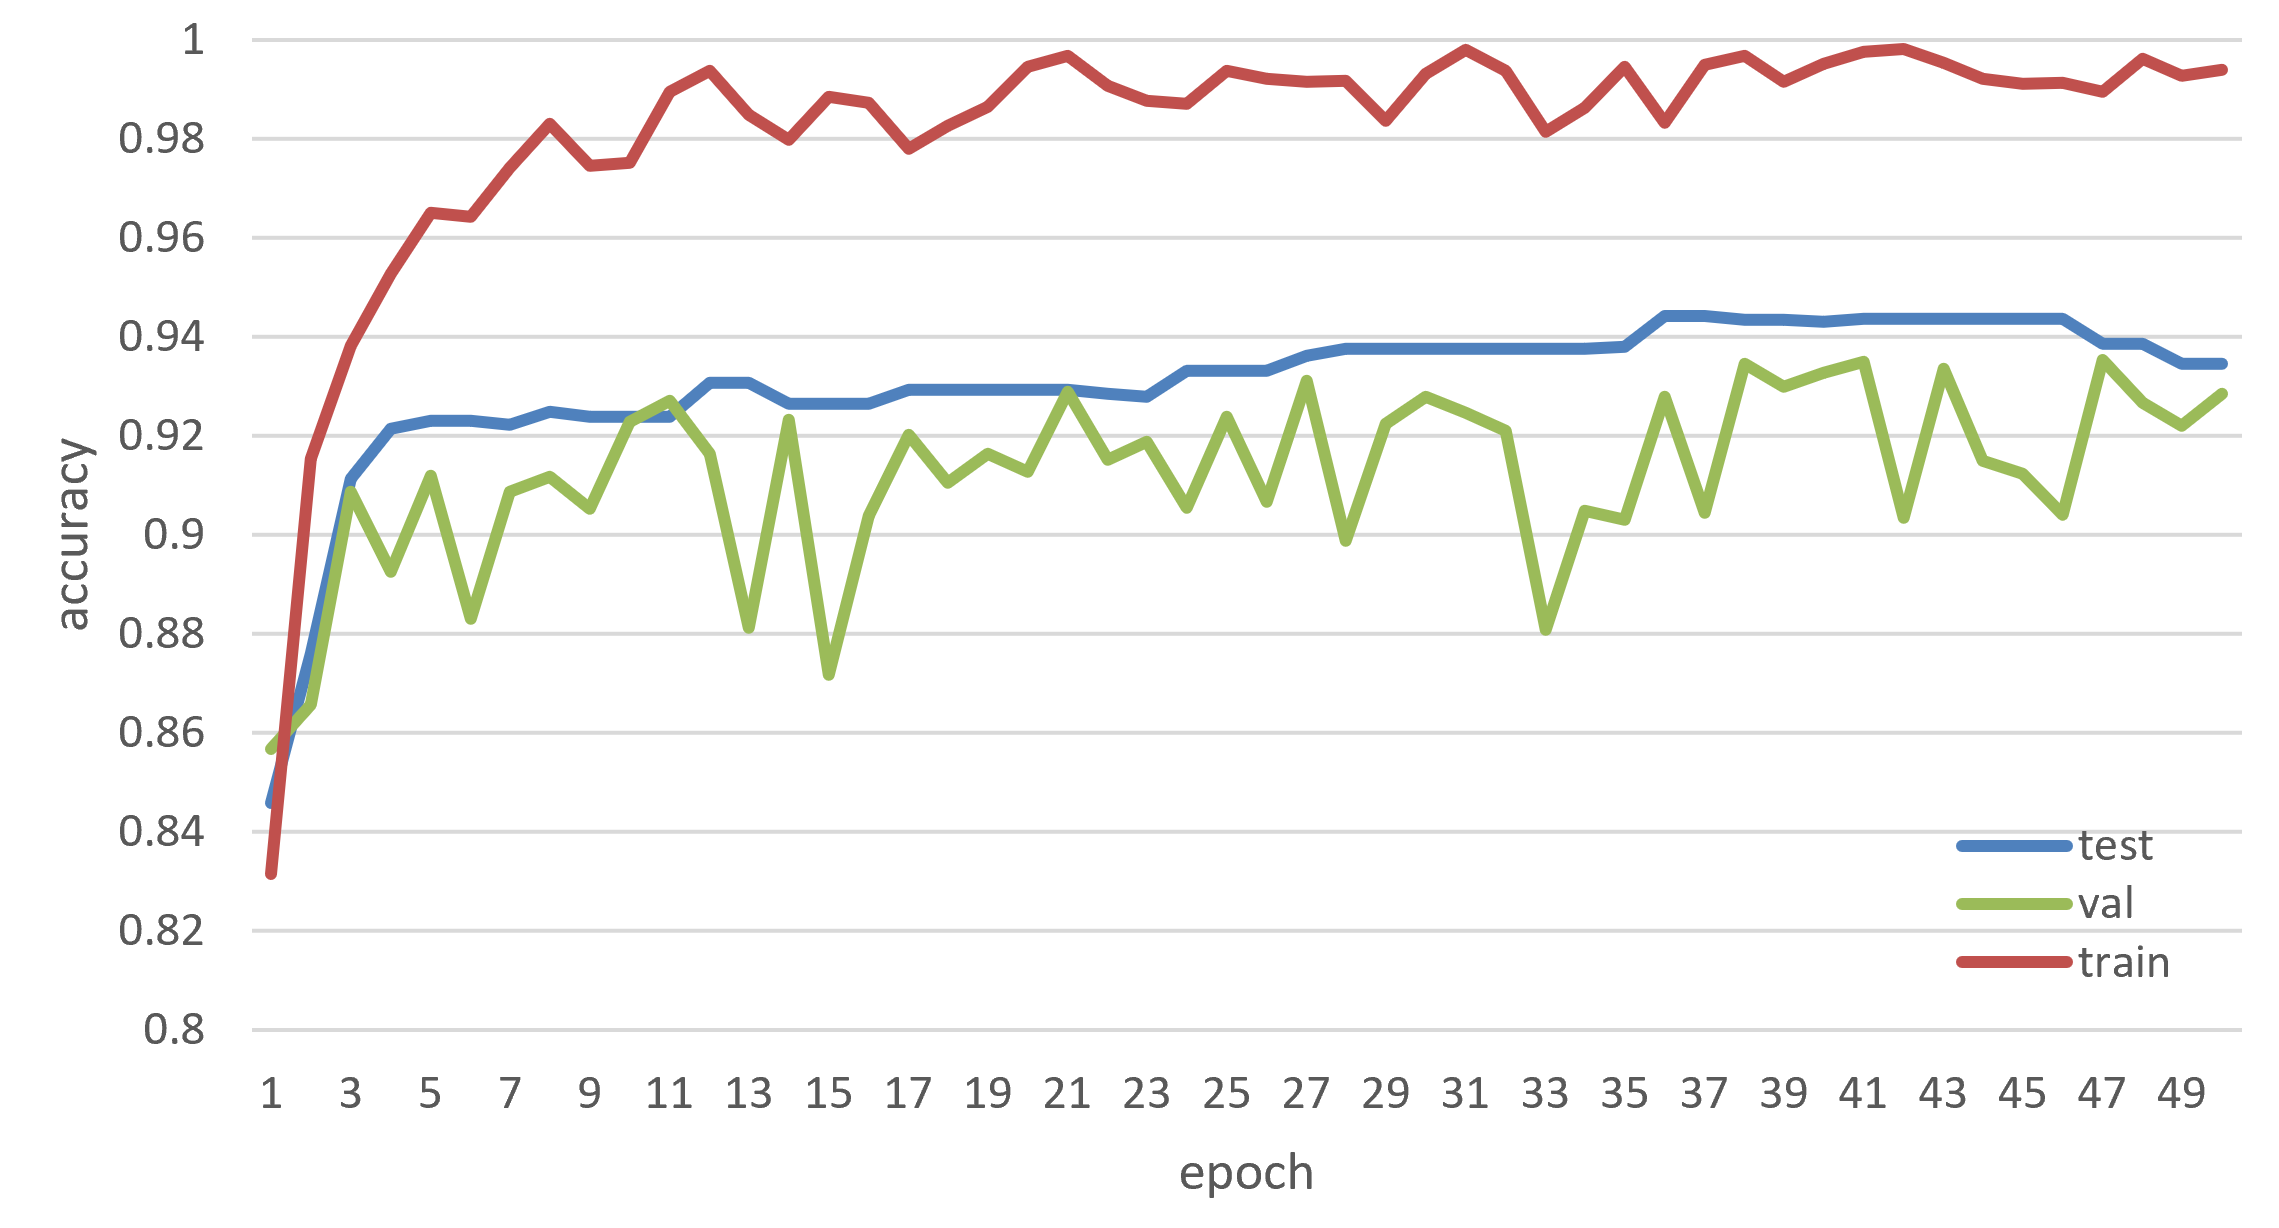
\includegraphics[scale=0.26]{images/baseline_resnet18_1round_acc.png}
    \caption{Training, validation and test accuracy of baseline (with ResNet-18 encoder) to the number of training epochs in one of 5-fold cross-validation.}
    \label{fig:baseline_training_epoch}
\end{figure}

\subsection{Contrastive Self-Supervised Training}
\label{sec:contrastive_ssl_ex}
We utilize ResNet-34 as the encoder and pretrain MoCo v2. BYOL and Barlow Twins for 300 epochs with a batch size of 96. After pretraining, we finetuning with encoder initialized by pretrained parameters for 50 epochs. The results of finetuning are shown in Table \ref{tab:finetune_methods}.
\begin{table}[tb]
\caption{Finetuning accuracy for MoCo v2 BYOL and Barlow Twins. The encoder is ResNet35.}
\centering
\begin{tabular}{l|l}
\hline
Methods    & Accuracy (\%) \\ \hline
MoCo v2    & 90.6          \\
BYOL       & 93.2           \\
Barlow Twins     & 91.5   \\
\hline   
\end{tabular}
\label{tab:finetune_methods}
\end{table}

It can be seen from Table \ref{tab:finetune_methods} that BYOL gets best performance in three self-supervised methods. It is intriguingly to find that MoCo v2 get relative lower performance. The reason may be due to the large number of positive samples considered as negative samples in binary classification tasks. This issue will be further investigated in \ref{sec:disscussion_moco}.

According to studies on contrastive self-supervised learning, the batch size, encoder size, and number of pretraining epochs could all have a significant impact on performance. 
According to the result of baseline experiment, smaller encoder could have better performance. Therefore, based on BYOL, we compare the performance with different encoder, epochs and batch size. The results are shown in Table \ref{tab: optimization of epoch,batchsize, size of encoder} which also includes the baseline results for comparison. 

\begin{table}[t]
\centering
\caption{Optimization of epochs, batchs size and size of encoder of pretraining. Where accuracy exceeds the baseline, it is highlighted in red. BYOL is used as pretraining method.}
\begin{tabular}{l|l|l|l}
\hline
encoder             & number of epoch & batch size & accuracy(\%)           \\ \hline
Baseline\_ResNet-18 & -               & -          & 93.8                        \\
Baseline\_ResNet-34 & -               & -          & 93.5                        \\ \hline
ResNet-34           & 300             & 96         & 93.2                        \\
ResNet-18           & 300             & 96         & 93.6                        \\
ResNet-18           & 600             & 256        & {\color[HTML]{FE0000} 94.0} \\
ResNet-18           & 300             & 256        & 93.6                    \\ \hline
\end{tabular}
\label{tab: optimization of epoch,batchsize, size of encoder}
\end{table}

From Table \ref{tab: optimization of epoch,batchsize, size of encoder}, about the size of encoder we can see that the performance is in line with baseline, that the smaller encoder performs better. Unlike in the contrastive self-supervised learning research on ImageNet, the larger encoder gets better performance does not work here. 
Furthermore, we discover that more epochs in BYOL pretraining can improve encoder training while larger batch size does not. When the ResNet-18 is pretrained after 600 epochs with 256 batch size, its performance outperforms the baseline which is inspiring. This result prove that contrastive self-supervised learning can improve the performance of Crohn's disease detection. However, there is still a lot of room for improvement. Since our primary goal is to investigate whether contrastive self-supervised learning is effective for Crohn's disease detection and which kind of contrastive method is more effective, we haven't done much tuning of the network structure and training parameters. We believe that many operations, such as training for longer epochs, using smaller encoders and simpler MLP layers, and using more specifically aimed data augmentation for WCE images could improve performance.

\subsection{Evaluation During Contrastive Pretraining}
\begin{figure}[tb]
    \centering
    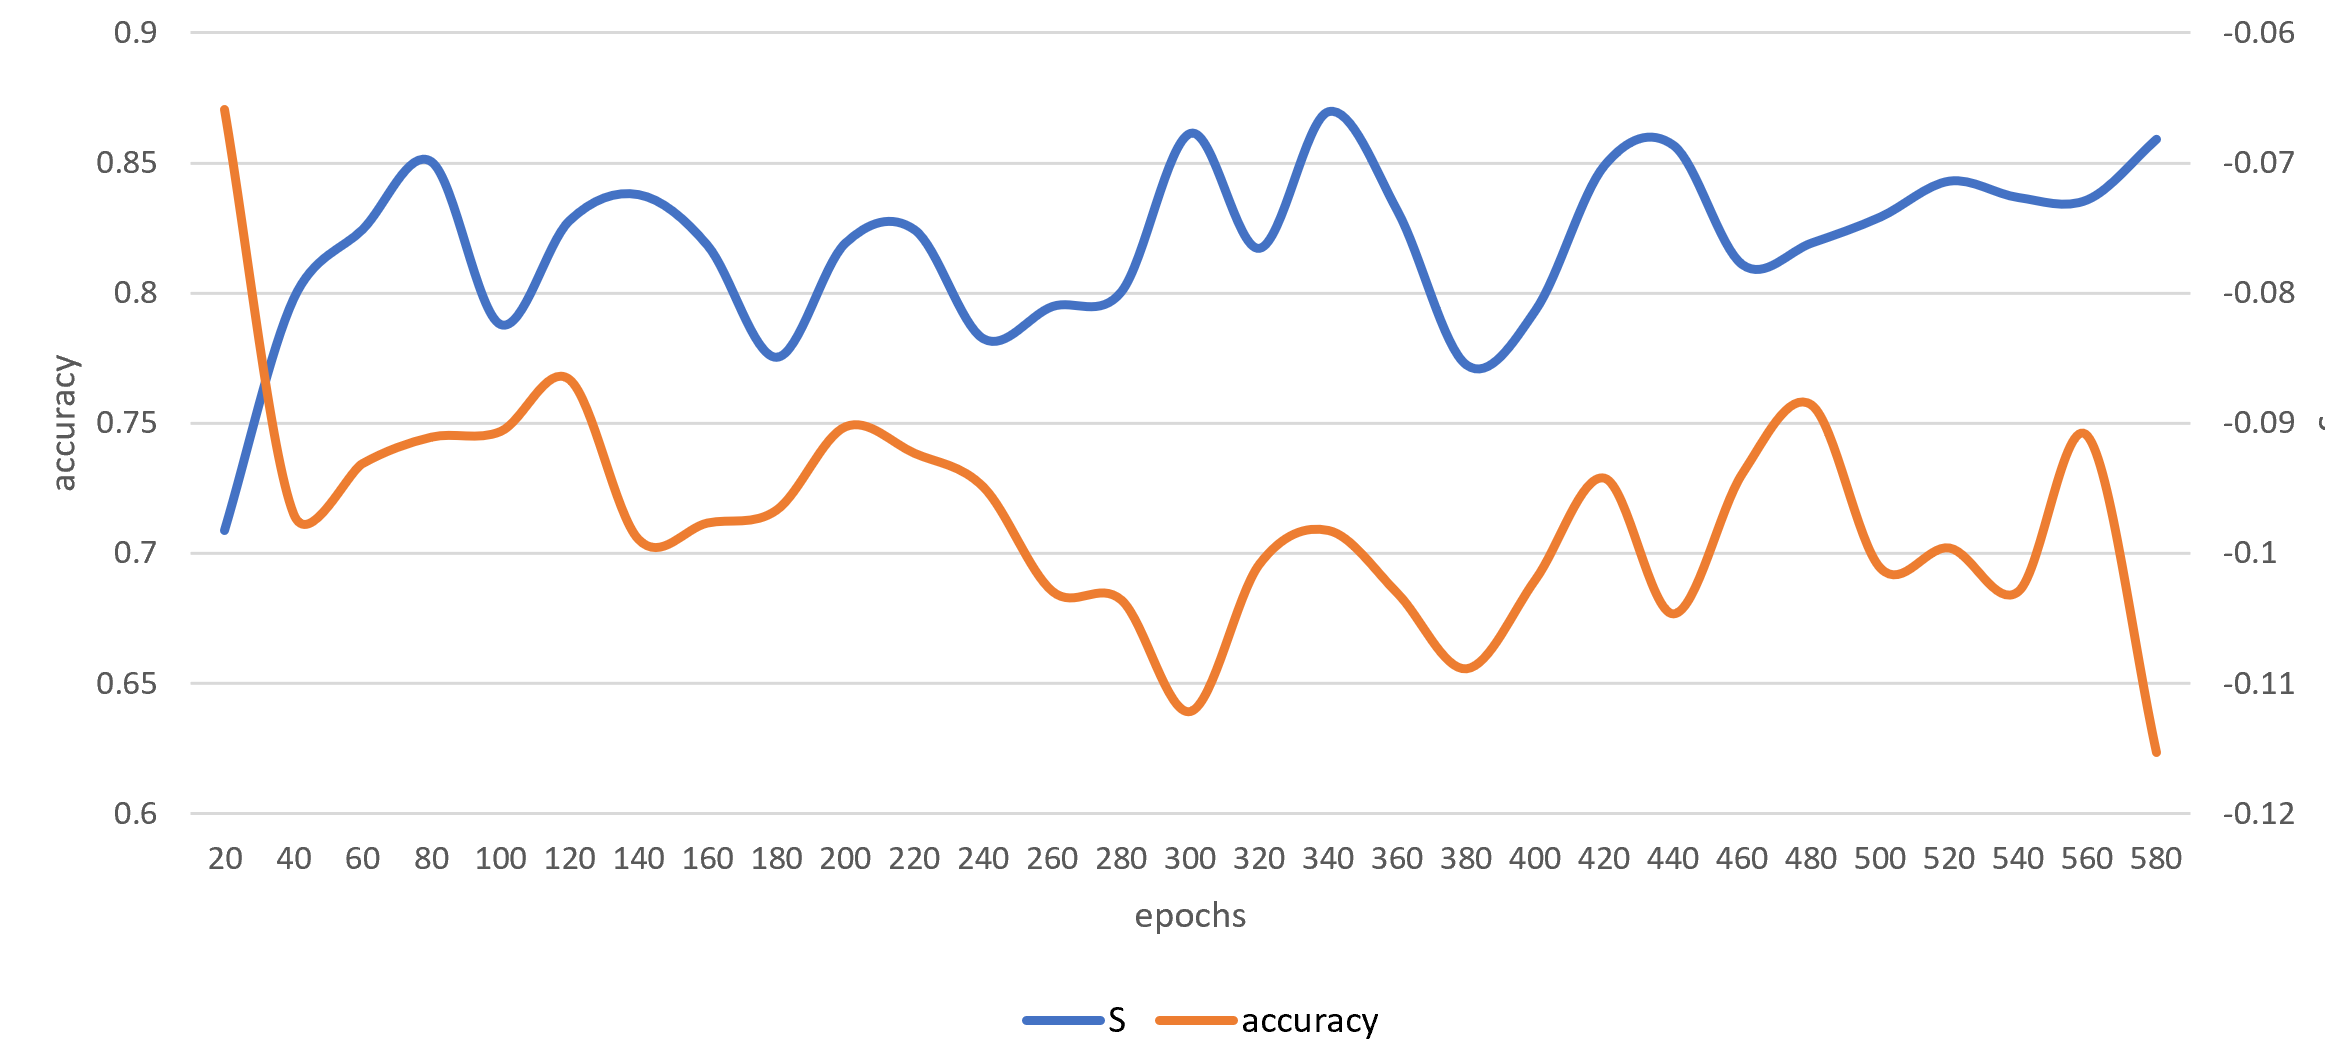
\includegraphics[scale=0.27]{images/edcp.png}
    \caption{The curve of one-epoch-finetuning accuracy and distance $S$ of ECDP during pretraining. $S$ is $S_{EDCP}$ in \eqref{equ:eval_distance1}.}
    \label{fig:evaluation tool}
\end{figure}
When the encoder is better pretrained, the accuracy of one-epoch-finetuning should increase, while the representation distance of positive samples decreases and the distance between negative sample pairs increases, resulting in a decrease in $s_{EDCP}$. The results of EDCP and one-epoch-finetuning accuracy are shown in Fig. \ref{fig:evaluation tool}. The curves of Fig. \ref{fig:evaluation tool} shows that the trends in accuracy and $s_{EDCP}$ are roughly opposite. When the training reaches 300 epoch, for example, the accuracy and $s_{EDCP}$ reach a local maximum and a local minimum, respectively. Besides, from the overall downward trend of $s_{EDCP}$, we can also know that the performance increases with the increase of the number of epochs, and has not converged, which is consistent with the results shown in the Table \ref{tab: optimization of epoch,batchsize, size of encoder}.
As a result, the curve demonstrates that $s_{EDCP}$ can effectively reflect the training degree during the pretraining process and can be used as an early-stopping and encoder selection tool in pretraining.

\section{Disscussion}
\subsection{Noisy Negative Samples of MoCo v2}
\label{sec:disscussion_moco}
According to study in MoCo\cite{he2019moco}, increasing the number of features taken from the memory bank improves performance, similar to increasing the batch size in SimCLR. However, in our experiment, MoCo v2 does not perform well when there are a large number of negative sample pairs, according to the results shown in \ref{sec:contrastive_ssl_ex}. 
We believe that it is due to the noisy sample pairs, in which many positive samples are misidentified as negative samples. 
Because MoCo is an instance-instance contrastive self-supervised learning method. 
During pretraining, all other samples are negative samples for a sample. This strategy, however, is harmful for binary classification tasks. 
Because there will be a large number of samples that are considered negative during pretraining but positive during finetuning. 
This causes the encoder to undergo conflicting training and it becomes more severe as the number of negative samples increases when pretraining.
There is no such issue in BYOL or Barlow Twins. Because BYOL does not use negative samples, and the negative samples used by the Barlow Twins are based on filters. The results of Table \ref{tab:dis_memorybank} show that reducing the number of negative samples improves the performance of MoCo v2 on Crohn's detection significantly.
As a result, the sample-based contrastive self-supervised method may not be appropriate for binary classification or tasks on small dataset. Furthermore, the noise cancellation for samples merits further investigation.
\begin{table}
\centering
\caption{Memory bank comparison}
\label{tab:dis_memorybank}
\begin{tabular}{l|l} 
\hline
Memory bank & accuracy(\%)  \\ 
\hline
576         & 91.5          \\
65536       & 90.6          \\
\hline
\end{tabular}
\end{table}



\subsection{Self-Supervised Learning on Small Dataset}
Research on self-supervised methods is generally conducted on large benchmarks, such as ImageNet, because this provides a more objective evaluation of models and methods.
Nevertheless, in the field of medical images, many datasets are small and the data diversity is limited due to the focus on specific disease or body part, such CrohnIPI. 
As a result, some methods and techniques that work on ImageNet may not work on small datasets.
For instance, while a larger encoder and batch size are typically effective in improving performance on ImageNet, they are ineffective and even worsen performance in our experiments.
Network and training strategy design for small datasets is lacking. These methods are critical in the practical application of deep learning methods, such as classification and segmentation of various medical image tasks. We hope that this study inspires more research into self-supervised learning on small datasets and we will also continue to investigate the application of self-supervision on small data sets.

\section{conclusion}
To alleviate the lack of sufficient labeled data for Crohn's disease detection, we investigated the use of contrastive self-supervised learning methods combined with unlabeled data, which improved the accuracy to 94\%.  We also propose an evaluation during contrastive pretraining (EDCP) method for monitoring pretraining and model selection for self-supervised pretraining. Finally, we observed some intriguing issues with using contrastive self-supervised learning for small dataset tasks in our experiments that merit further investigation.



\bibliography{bib}
\bibliographystyle{IEEEtran}


\end{document}
